
\newpage
\appendix
\section{Appendix A} \label{AppendixA}
% the \\ insures the section title is centered below the phrase: AppendixA

\subsection{Detailed Paths Analysis in Triple Loops} 

Now let us consider the different routes to each target in $6$ cases depending on the location of the {\it black virus}.  Let $\pi[x_0,x_{i}] $ denote a path to reach target $x_i$, and let $dif=k-p$, we have the following situations:
\begin{itemize}
\item {\bf Case1}: Let us study the case of finding the \bv in the third segment of the chordal ring: $k\leq |S_{area}| <n-k$. In this case, triggering the original \bv creates three more \bvs: $x_{1}$, $x_{p}$ and $x_{k}$, and thus $\cal T$=$\{x_{2}$, $x_{p-1}$, $x_{p-k}$, $x_{k-1}$, $x_{p+1}$, $x_{k+1}$, $x_{k-p}$, $x_{k+p}$,  $x_{2p}$, $x_{2k}\}$. 
\begin{itemize}

\item  $x_{k-1}$:  Node  $x_{k-1}$ is reached through  $\sigma_{k-1}$
 
$$ \sigma_{k-1} =  x_{0}\xrightarrow {-1}x_{-1}\xrightarrow {+k}x_{k-1}$$

%################################################################

\item  $x_{p-1}$:  Node  $x_{k-1}$ is reached through $\sigma_{p-1}$
 
$$ \sigma_{p-1} =  x_{0}\xrightarrow {-1}x_{-1}\xrightarrow {+p}x_{p-1}$$

%################################################################

\item $x_{2}$:  could be reached in different ways:\\
$$ \pi[x_0,x_{2}] = \min \{ \pi_1, \pi_2,  \pi_3,\}$$


 \begin{itemize} 
 
\item  taking advantage of the fact that $x_{-k}$ is known to be safe: 
%the target is reached in 4 moves as follows:
$$ \pi_{1}  =   x_{0}\xrightarrow {-k}x_{-k} \xrightarrow {+1}x_{1-k}\xrightarrow {+1}x_{2-k}\xrightarrow {+k}x_{2}$$
\item  taking advantage of the fact that $x_{-p}$ is known to be safe: 
%the target is reached in 4 moves as follows:
$$ \pi_{2}  =   x_{0}\xrightarrow {-p} x_{-p} \xrightarrow {+1}x_{1-p}\xrightarrow {+1}x_{2-p}\xrightarrow {+p} x_{2}$$
\item If  $p = 4$ %the target is reached in 3 moves by :
$$ \pi_3  =   x_{0}\xrightarrow {-1}x_{-1} \xrightarrow {+p}x_{p-1}\xrightarrow {-1}x_{2}$$
\item If $p = 3$ %the target reached in two moves:
$$   \pi_3 =  x_{0}\xrightarrow {-1}x_{-1} \xrightarrow {+p}x_{2}$$
\end{itemize}
%################################################################
\item x $_ {p+1}$:


 \begin{itemize} 
\item Taking advantage of the fact that $x_{-k}$ is known to be safe:
$$ \pi_{4} = x_{0} \xrightarrow {-k} x_{-k} \xrightarrow {+p} x_{-k+p}\xrightarrow {+1} x_{-k+p+1}\xrightarrow {+k} x_{p+1} $$


%$$ \sigma_{p+1} = x_{0} \xrightarrow {-1} x_{-1} \xrightarrow {+p} x_{p-1}\xrightarrow {+p} x_{2p-1}\xrightarrow {+1} x_{2p} \xrightarrow {+1} x_{2p+1}\xrightarrow {-p} x_{p+1}$$

 \item If $k=2p$
$$ \pi_5 = x_{0} \xrightarrow {-p} x_{-p} \xrightarrow {+1} x_{-k+p+1}\xrightarrow {+k} x_{p+1} $$

\item  If $k=2p+1$
$$ \pi_5 = x_{0} \xrightarrow {-p} x_{-k+p+1} \xrightarrow {+k} x_{p+1} $$
\end{itemize}
%################################################################


 \item x$_ {k-p}$: %the neighbour that is connected to x $_ {k}$ through the $-p^{th}$ %chord; of course this node \textgreater x$_ {0}$.
%\begin {center}
%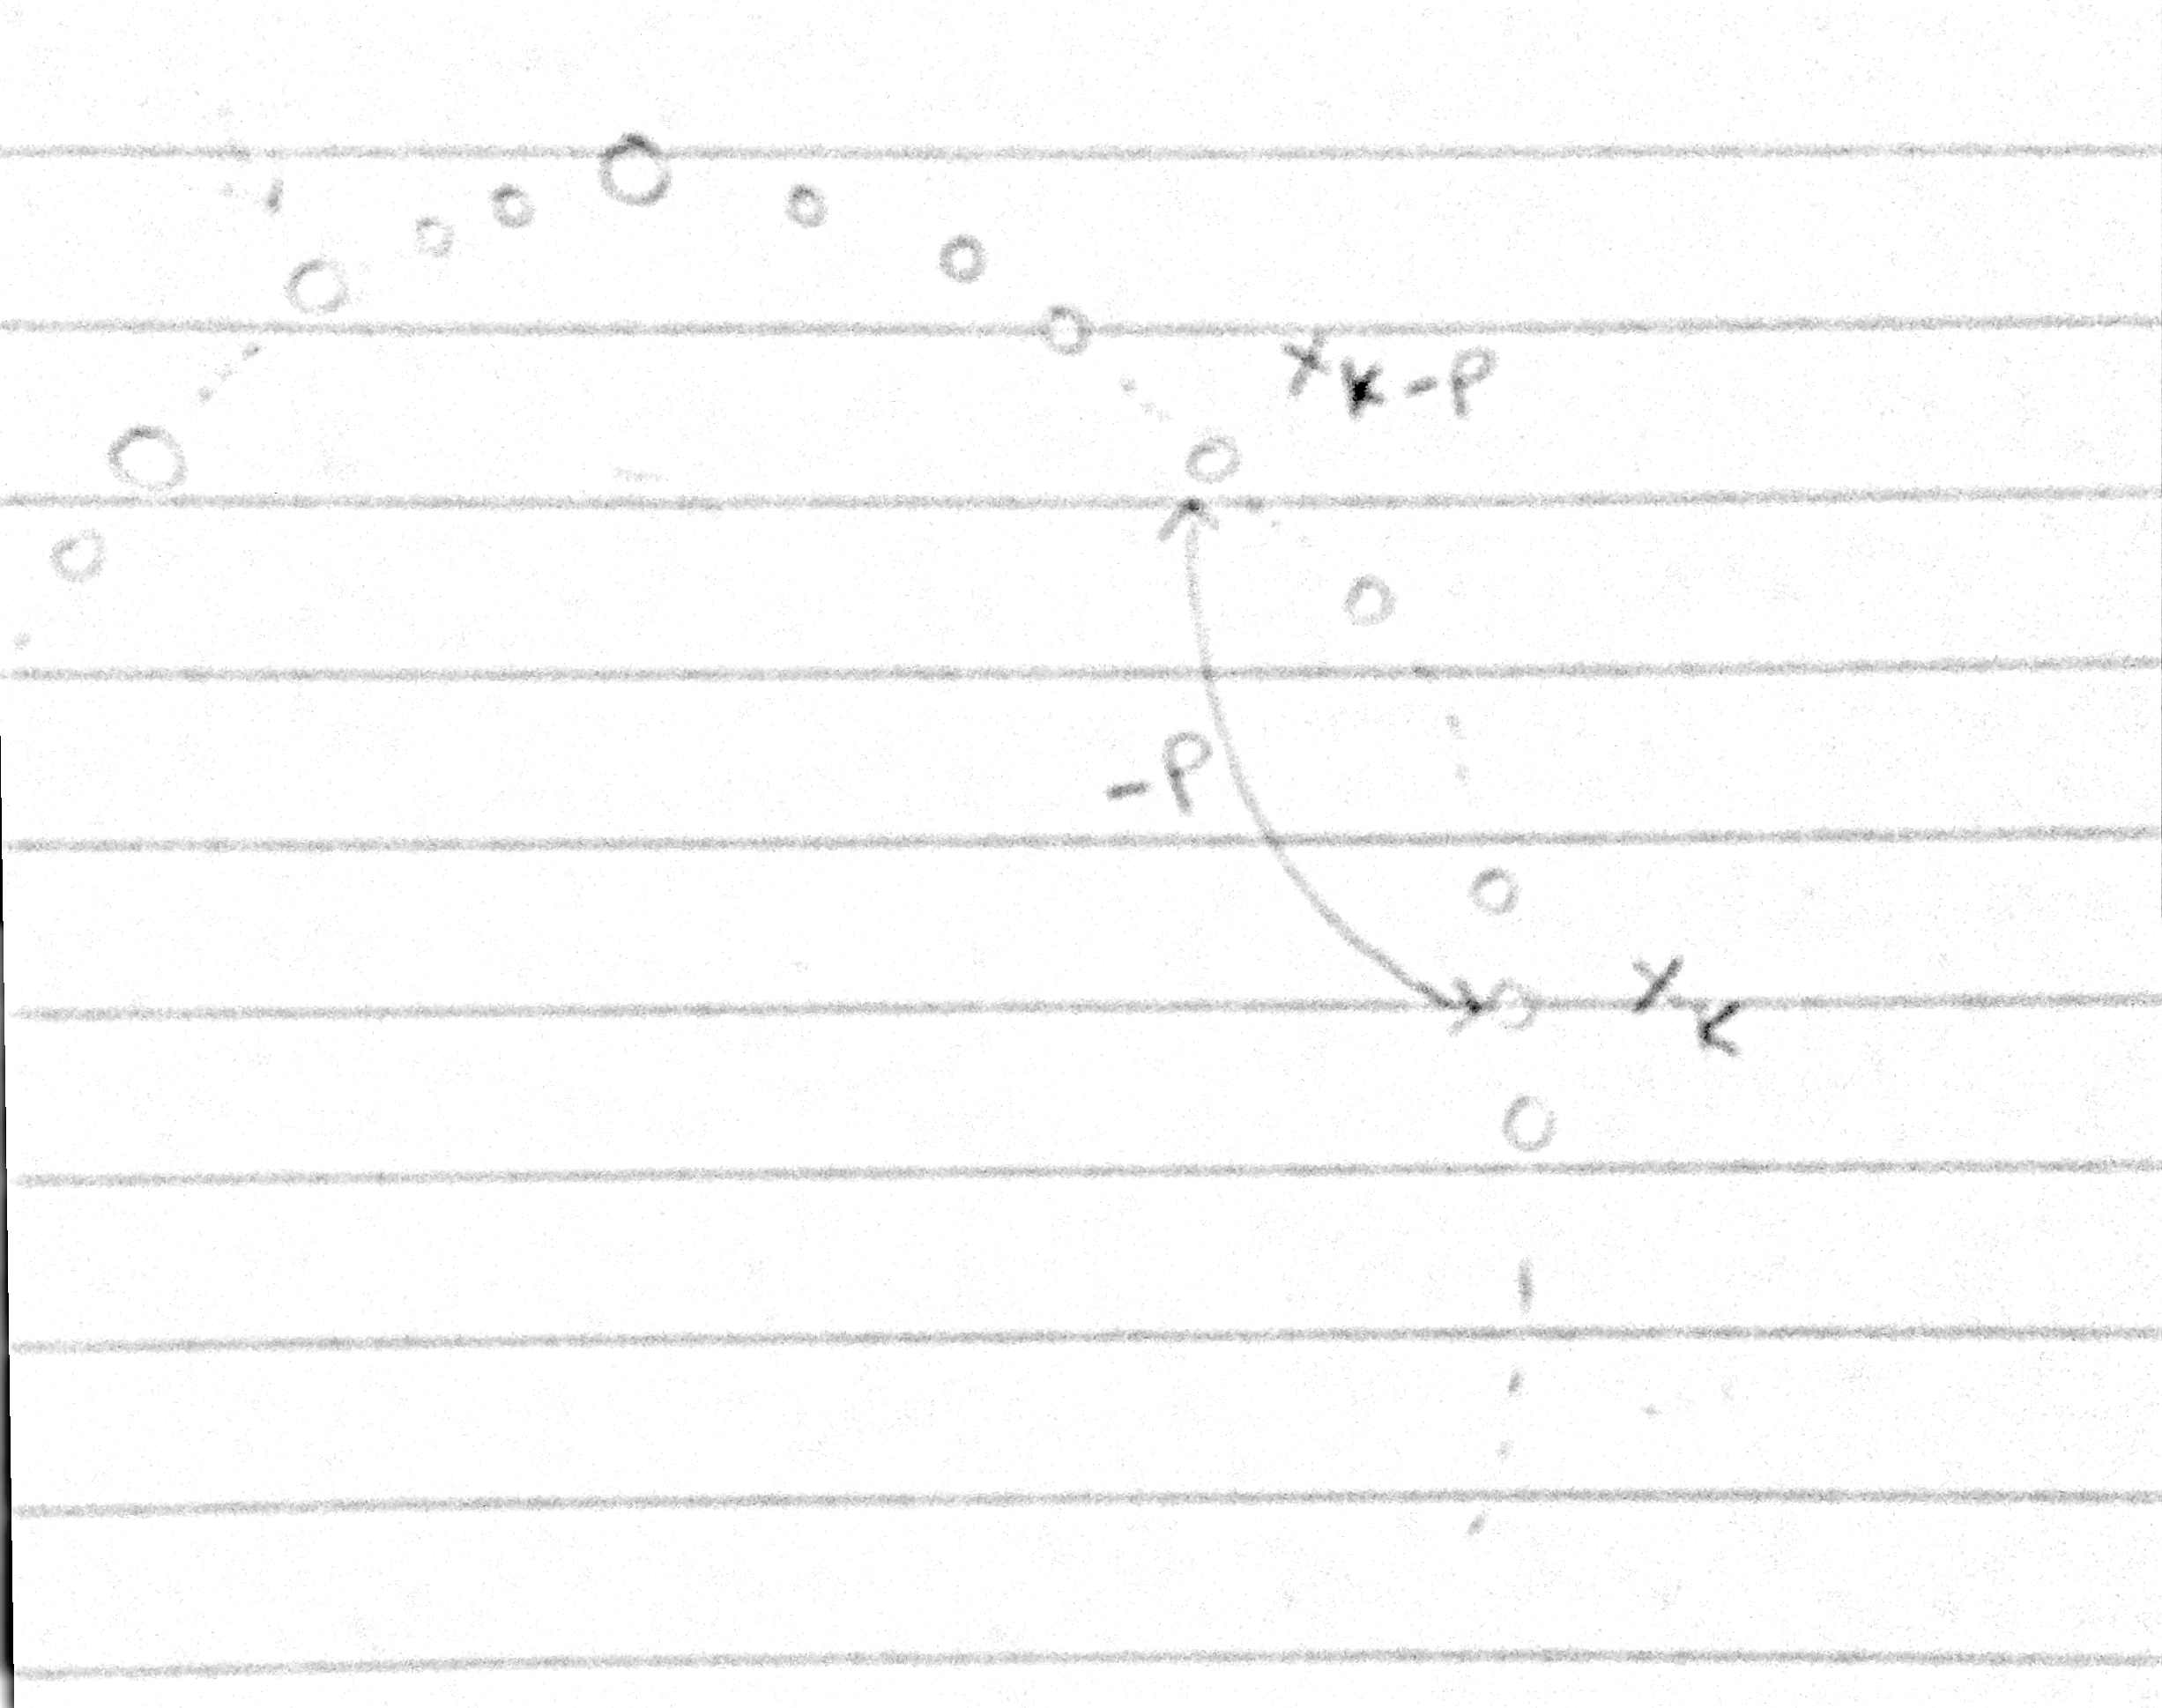
\includegraphics [scale=0.10] {xk-p.jpg}
%\end {center}
%Notice that when $p > dif$,  $p-1 \ge k-p$, so:
%\\the number of moves between x$_ {p-1}$ and x$_ {k-p} = 2p-k-1 $  (p-1-(k-p))
$$ \pi[x_0,x_{k-p}] = \min \{ \pi_6, \sigma_{k-p}\}$$
where
$$\sigma_{k-p} =x_{0} \xrightarrow {-1} x_{-1} \xrightarrow {+k} x_{k-1} \xrightarrow {-p} x_{k-p-1}\xrightarrow {+1} x_ {k-p}$$

$\pi_6=$


 
\begin{itemize}
\item If $k<2p$
 $$  x_{0} \xrightarrow {-1} x_{-1} \xrightarrow {+p} x_{p-1} \xrightarrow {-1} x_{p-2}...\xrightarrow {-1} x_ {k-p}$$
%\\the total $= 2p-k-1+2 =2p-k+1 $ 
\item If $p = dif$, there is no x$_ {k-p}$.
\item Else, x$_ {k-p}$ is between x$_ {p}$ and x$_ {k}$. %% between second and %%third

%\\Notice that when $p < dif$,  $k > k-p$, so:
%\\the number of moves between x$_ {k-1}$ and x$_ {k-p} = p-1 $  (k-1-(k-p))
$$ x_{0} \xrightarrow {-1} x_{-1} \xrightarrow {+k} x_{k-1} \xrightarrow {-1} x_{k-2}...\xrightarrow {-1} x_ {k-p}$$
%\\the total $= p-1+2 =p+1 $ 
\end{itemize}
If applicable(i.e., $k\neq 2p+1$)


%################################################################

\item $x_{2p}$ is reached through $\sigma_{2p}$:

$$\sigma_{2p} = x_{0} \xrightarrow {-1} x_{-1} \xrightarrow {+p} x_{p-1} \xrightarrow {+p} x_{2p-1}\xrightarrow {+1} x_{2p} $$

%################################################################




\item $x_{2k}$ is reached through $\sigma_{2k}$:
 
$$\sigma_{2k} = x_{0} \xrightarrow {-1} x_{-1} \xrightarrow {+k} x_{k-1} \xrightarrow {+k} x_{2k-1} \xrightarrow {+1}  x_{2k}$$

%################################################################

\item$x_{k+1}$:
$$ \pi[x_0,x_{k+1}] = \min \{ \pi_7, \sigma_{k+1},\pi_8,\pi_9\}$$
where

$$  \sigma_{k+1} =   x_{0} \xrightarrow {-1} x_{-1} \xrightarrow {+k} x_{k-1} \xrightarrow {+k} x_{2k-1}
 \xrightarrow {+1}  x_{2k}\xrightarrow {+1} x_{2k+1} \xrightarrow {-k} x_{k+1}$$

$\pi_7=$

 \begin{itemize}
\item If $k<2p$
$$    x_{0} \xrightarrow {-1} x_{-1} \xrightarrow {+p} x_{p-1} \xrightarrow {+p} x_{2p-1}
 \xrightarrow {-1}  x_{2p-2} \xrightarrow {-1},..., \xrightarrow {-1} x_{k+1}$$
\item If $k>2p$
$$    x_{0} \xrightarrow {-1} x_{-1} \xrightarrow {+p} x_{p-1} \xrightarrow {+k} x_{k+p-1}
 \xrightarrow {-i}  x_{k+p-i} ,..., x_{k+1}$$
where $i=1$ or $i=p$ depending on whether the differnece between $x_{k+1}$ and $x_{k+p-1}$ is greater than $p$ or not.
\end{itemize}
If $ |\pi[x_0,x_{k-p}]| <4$, then  x$_{k+1}$ is reached through $\pi_6$  plus two more moves.

$$\pi_8= \pi_6 + x_{k-p}\xrightarrow {+1} x_{k-p+1} \xrightarrow {+p}x_{k+1}$$

If $ |\pi[x_0,x_2]| <4$, then  x$_{k+1}$ is reached through $\pi_3$  plus two more moves.
$$\pi_9= \pi_3 + x_{2}\xrightarrow {+k} x_{k+2} \xrightarrow {-1} x_{k+1}$$



% or -1,1-,1-k+p,-1(p-k),-1(p-k-1),...,1+k # of moves p+1
%################################################################


\item $x_{k+p}$ is reached through $\sigma_{k+p}$:
$$\sigma_{k+p}= x_{0}\xrightarrow {-1} x_{-1}\xrightarrow {+p} x_{p-1} \xrightarrow {+k} x_{k+p-1}\xrightarrow {+1} x_{k+p}$$%, 4 moves


%################################################################



\item $x_{p-k}$ 
$$ \pi[x_0,x_{p-k}] = \min \{ \pi_{10}, \sigma_{p-k}\}$$
where
$$\sigma_{k+p}= x_{0}\xrightarrow {-1} x_{-1}\xrightarrow {+p} x_{p-1} \xrightarrow {-k} x_{p-k-1}\xrightarrow {+1} x_{p-k}$$%, 4 moves
$\pi_{10}=$
\begin{itemize}
\item If $dif \leq 3$
$$ x_{0}\xrightarrow {-1} x_{-1}\xrightarrow {-1} x_{-2} ,...,\xrightarrow {-1} x_{p-k}$$
\item If $p \leq 3$
$$ x_{0}\xrightarrow {-k} x_{-k}\xrightarrow {+1} x_{-k+1} \xrightarrow {+1} ,...,\xrightarrow {+1} x_{p-k}$$
\item If $p-dif<3$
$$ x_{0}\xrightarrow {-p} x_{-p}\xrightarrow {+1} x_{-p+1} \xrightarrow {+1} ,...,\xrightarrow {+1} x_{p-k}$$

\end{itemize}
%$$ x_{0}\xrightarrow {-p} x_{-p}\xrightarrow {-1} x_{-p-1} \xrightarrow {-1} ,...,\xrightarrow {-1} x_{p-k}$$
%$$ x_{0}\xrightarrow {-k} x_{-k}\xrightarrow {+1} x_{-k+1} \xrightarrow {+1} ,...,\xrightarrow {+1} x_{p-k}$$
%$$ x_{0}\xrightarrow {-k} x_{-k}\xrightarrow {+i} x_{-k+i},..., x_{p-k}$$
%################################################################
\item Nodes $x_{-p+1}$, and $x_{-k+1}$ are occupied by $SH$s that were at nodes  $x_{-p}$ and $x_{-k}$ respectively when the original \bv got triggered.. 
\end{itemize}
We have to take into consideration the fact that some of the above paths might be not applicable if they pass thorough a $BV$. However, the special paths are always applicable.
%******************************************************************************************
%******************************************************************************************

 \item {\bf Case2}: In the case of finding the \bv in the fourth segment $n-k\leq |S_{area}| <n-p$, two \bvs are generated, which are at $x_1$ and $x_p$, since the rest neighbours are explored and guarded. Thus,
$\cal T$=$\{x_2,x_{p-1},x_{p+1}x_{p-k}x_{p+k}x_{2p}\}$
\begin{itemize}
\item $x_2$ is reached using $\pi_1$ or $\pi_2$ or$\pi_3$ as we discussed in {\bf Case1}.
\item $x_{p-1}$ is reached using $\sigma_{p-1}$
\item $x_{p+1}$ is reached using $\pi_4$ or $\pi_5$  as we discussed in {\bf Case1}.
\item $x_{p-k}$ is reached using $\sigma_{p-k}$ or $\pi_{10}$ as we discussed in {\bf Case1}.
\item $x_{p+k}$ is reached using $\sigma_{p+k}$.
\item $x_{2p}$ is reached using $\sigma_{2p}$.
\item $x_{k+1}$, $x_{-p+1}$, and $x_{-k+1}$ are occupied by $SH$s that were at nodes $x_{k}$, $x_{-p}$ and $x_{-k}$ respectively when the original \bv got triggered. 
\end{itemize}

%******************************************************************************************
%******************************************************************************************
\item {\bf Case3}: In the case of finding the \bv in the fifth segment $n-p\leq |S_{area}| <n-1$, one \bv is generated, which is at $x_1$ since the rest neighbours are explored and guarded. Thus,
$\cal T$=$\{x_2\}$ 
\begin{itemize}
\item $x_2$ is reached using $\pi_1$ or $\pi_2$ or$\pi_3$ as we discussed in {\bf Case1}.

\item Nodes $x_{p+1}$, $x_{k+1}$, $x_{-p+1}$, and $x_{-k+1}$ are occupied by $SH$s that were at nodes $x_{p}$, $x_{k}$, $x_{-p}$ and $x_{-k}$ respectively when the original \bv got triggered. 
\end{itemize}


%******************************************************************************************
%******************************************************************************************
\item {\bf Case4}: We have a special case when the \bv is located at node $n-1$. In this case, all neighbours are guarded and no more \bvs are created. No more moves are made in the second phase since all moves are done in the first phase as we explained in the previous section.
%******************************************************************************************
%******************************************************************************************

\item {\bf Case5}: In the case of finding the \bv in the second segment $p\leq |S_{area}| <k$, four \bvs are generated, which are at $\cal BV$=$\{x_1,x_p,x_k,x_{-k}\}$ since only one $SH$ has been deployed so far at node $x_{-p}$. Thus,
$\cal T$=$\{x_{2}$, $x_{p-1}$,  $x_{k-1}$, $x_{p+1}$, $x_{k+1}$, $x_{k-p}$, $x_{k+p}$, $x_{2p}$, $x_{2k}$, $x_{-k+p}$, $x_{-k+1}$, $x_{-k-1}$, $x_{-k-p}$, $x_{-2k}\}$. To reach any of these targets, we should avoid any path that has $x_{-k}$.
\begin{itemize}
\item Node $x_{2}$ is reached as the following:  
$$ \pi[x_0,x_{2}] = \min \{ \pi_2,\pi_3\}$$

\item Node $x_{p-1}$ is reached using $\sigma_{p-1}$ 

\item Node $x_{k-1}$ is reached using $\sigma_{k-1}$ 

\item Node $x_{p+1}$ is reached as the following:  
$$ \pi[x_0,x_{p+1}] = \min \{ \pi_5,\sigma_{p+1}\}$$

\item Node $x_{k+1}$ is reached as the following:  
$$ \pi[x_0,x_{k+1}] = \min \{ \pi_7,\pi_8,\pi_9,\sigma_{k+1}\}$$

\item Node $x_{k-p}$ is reached as the following:  
$$ \pi[x_0,x_{k-p}] = \min \{ \pi_6,\sigma_{k-p}\}$$


\item Node $x_{k+p}$ is reached using $\sigma_{k+p}$ 

\item Node $x_{2p}$ is reached using $\sigma_{2p}$ 

\item Node $x_{2k}$ is reached using $\sigma_{2k}$ 

\item Node $x_{-k+p}$ is reached as the following:  
$$ \pi[x_0,x_{-k+p}] = \min \{ \pi_{10},\sigma_{-k+p}\}$$

\item Node $x_{-k+1}$ is reached as the following:
$$ \pi[x_0,x_{-k+1}] = \min \{ \pi_{11},\sigma_{-k+1}\}$$
where 
$$ \pi_{11} = x_{0} \xrightarrow {-1} x_{-1} \xrightarrow {-p} x_{-p-1} \xrightarrow {-i},...\xrightarrow {-i},x_{-k+1}  $$
where $i=1$ or $i=p$ depending on the distance $dist$ between $x_{-p-1}$ and $x_{-k+1}$. If $dist \ge p$, then $i=p$, otherwise, $i=1$.\\


\item Node $x_{-k-1}$ is reached using $\sigma_{-k-1}$ 

\item Node $x_{-k-p}$ is reached using $\sigma_{-k-p}$ 

\item Node $x_{-2k}$ is reached using $\sigma_{-2k}$ 

\item Node $x_{-p+1}$ is already guarded by a $SH$ that was at node $x_{-p}$ when the original \bv got triggered.


\end{itemize}

%******************************************************************************************
%******************************************************************************************

\item {\bf Case6}. Finding the \bv in the first segment $1\leq |S_{area}| <p$, five \bvs are generated, which are at $\cal BV$=$\{x_1,x_p,x_k,x_{-p},x_{-k}\}$ since no $SH$s have been deployed yet-p. Thus,
$\cal T$=$\{x_{2}$, $x_{p-1}$,  $x_{k-1}$, $x_{p+1}$, $x_{k+1}$, $x_{k-p}$, $x_{k+p}$, $x_{2p}$, $x_{2k}$, $x_{-p+1}$, $x_{-p-1}$, $x_{-2p}$,$x_{-k+p}$, $x_{-k+1}$, $x_{-k-1}$, $x_{-k-p}$, $x_{-2k}\}$. To reach any of these targets, we should avoid any path that has $x_{-p}$ or $x_{-k}$ as the following:
\begin{itemize}
\item Node $x_{2}$. Since $x_{-p}$ and $x_{-k}$ are $BV$s, we have
$$ \pi[x_0,x_{2}] = \min \{ \pi_{12},\sigma_{2}\}$$
where

$$\pi_{12}= x_{0} \xrightarrow {-1} x_{-1} \xrightarrow {+p} x_{p-1} \xrightarrow {-1}  x_{p-2} ... \xrightarrow {-1}  x_{2}$$ 

$$\sigma_{2}=x_{0} \xrightarrow {-1} x_{-1} \xrightarrow {+k} x_{k-1} \xrightarrow {+k} x_{2k-1} \xrightarrow {+1} x_{2k}  \xrightarrow {+1} x_{2k+1} \xrightarrow {+1} x_{2k+2} \xrightarrow {-k} x_{k+2} \xrightarrow {-k} x_{2}$$

\item Node $x_{p-1}$ is reached using $\sigma_{p-1}$ 

\item Node $x_{k-1}$ is reached using $\sigma_{k-1}$ 

\item Node $x_{p+1}$ is reached using $\sigma_{p+1}$ 


\item Node $x_{k+1}$ is reached as the following:  
$$ \pi[x_0,x_{k+1}] = \min \{ \pi_7,\pi_8,\pi_9,\sigma_{k+1}\}$$

\item Node $x_{k-p}$ is reached as the following:  
$$ \pi[x_0,x_{k-p}] = \min \{ \pi_6,\sigma_{k-p}\}$$

\item Node $x_{k+p}$ is reached using $\sigma_{k+p}$ 

\item Node $x_{2p}$ is reached using $\sigma_{2p}$ 

\item Node $x_{2k}$ is reached using $\sigma_{2k}$ 

\item Node $x_{-p+1}$ is reached using $\sigma_{-p+1}$ 

\item Node $x_{-p-1}$ is reached using $\sigma_{-p-1}$ 

\item Node $x_{-2p}$ is reached using $\sigma_{-2p}$ 

\item Node $x_{p-k}$ is reached as follows:  
$$ \pi[x_0,x_{p-k}] = \min \{ \pi_{10},\sigma_{p-k}\}$$
where
$$\pi_{10}= x_{0}\xrightarrow {-1} x_{-1}\xrightarrow {-1} x_{-2} ,...,\xrightarrow {-1} x_{p-k}$$

\item Node $x_{-k+1}$ is reached as follows:
$$ \pi[x_0,x_{-k+1}] = \min \{ \pi_{11},\sigma_{-k+1}\}$$

\item Node $x_{-k-1}$ is reached using $\sigma_{-k-1}$ 


\item Node $x_{-k-p}$ is reached using $\sigma_{-k-p}$ 

\item Node $x_{-2k}$ is reached using $\sigma_{-2k}$ 


\end{itemize}

%******************************************************************************************
%******************************************************************************************
\end{itemize}

\newpage
\section{\\Title of Appendix B} \label{App:AppendixB}
% the \\ insures the section title is centered below the phrase: Appendix B

Text of Appendix B is Here